\documentclass[aspectratio=169,professionalfonts, 12pt]{beamer}
\usepackage{lmodern}
\usepackage{array}
\usepackage{multirow}
\usepackage[french,english]{babel}
\usepackage[T1]{fontenc}
\usepackage{multicol}
\usepackage{ragged2e}   %new code
\usepackage[utf8]{inputenc}
\usepackage[brazil]{varioref}
\usepackage[square,sort,comma,super,authoryear]{natbib}
\usepackage{listings,xcolor}
\usepackage{xmpmulti}
\usepackage{epsfig}
\usepackage{subcaption}
\captionsetup{compatibility=false}
\usepackage{ru,graphicx,hyperref,url} % 
\usepackage{booktabs}
\usepackage{pgfplots}
\usepackage{tikz}
\usepackage{ amsmath, amssymb, amsfonts}
\addtobeamertemplate{block begin}{}{\justifying}
\setbeamertemplate{section in toc}[sections numbered]
\AtBeginSection[]
{
  \begin{frame}[t]
  \begin{multicols}{2}
      \tableofcontents[currentsection]
    \end{multicols}
  \end{frame}

}

\date{\today}
\definecolor{blueforest}{RGB}{00,74,09}
\begin{document}
\selectlanguage{french}
\begin{frame}[plain, noframenumbering]
	\titlepage
\end{frame}
\begin{frame}[plain,t, noframenumbering]
	\frametitle{Table des matières}
    \begin{multicols}{2}
    \tableofcontents
    \end{multicols}
\end{frame}

% Section titles are shown in at the top of the slides with the current section 
% highlighted. Note that the number of sections determines the size of the top 
% bar, and hence the university name and logo. If you do not add any sections 
% they will not be visible.
\section{INTRODUCTION}
\subsection{Contexte}
\begin{frame}
    \frametitle{Contexte}
    \justifying 
    \begin{minipage}{\textwidth}
    \begin{block}{}
    Les progrès fulgurants des Technologies de l’Information et de la Communication(TIC) et les nombreuses Innovations dans les communications réseaux ainsi que le besoin de faire collaborer des objets ont conduit à un concept moderne qui est l’Internet des objets(IoT).
    \end{block}
    	\only<1->
    \end{minipage} 
    \begin{minipage}{\textwidth}
    \onslide<2->
    	\begin{figure}[H]
        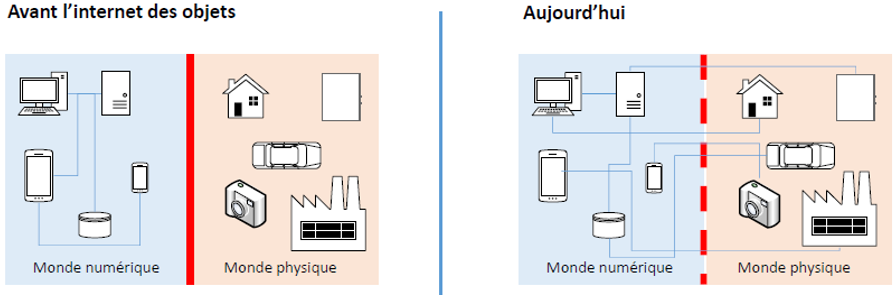
\includegraphics[ height=3.6cm]{images/mondeIoT}
      \end{figure}
    \end{minipage}
\end{frame}
\begin{frame}
\frametitle{Contexte(suite)}
	\justifying
    \begin{minipage}{\textwidth}
    \begin{block}{}
    Selon les experts de CISCO, le nombre d’objets connectés dans le monde est actuellement estimé à 30 milliards et ce nombre atteindrait les 75 milliards d’objets connectés en 2025. 
    \end{block}
    	\only<1->
    \end{minipage} 
    \textbf{}\\
    
    \textbf{}\\
    
    \textbf{}\\
    \begin{minipage}{\textwidth}
    \onslide<2->
    	\begin{figure}[H]
        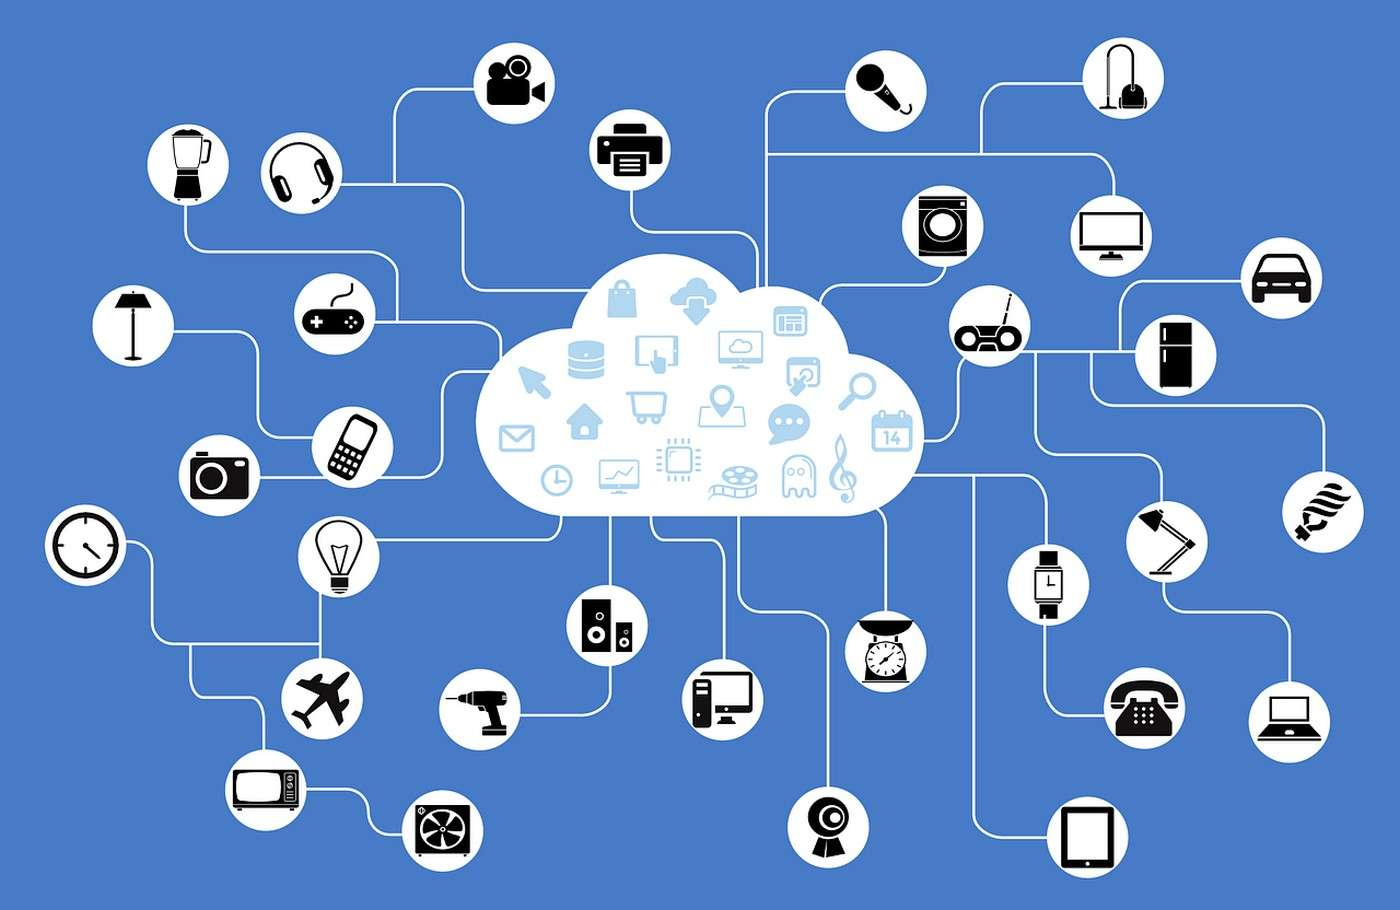
\includegraphics[height=0.5\textheight, width=0.6\textwidth]{images/Internet}
      \end{figure}
    \end{minipage}
\end{frame}
\subsection{Problématique}
\begin{frame}
    \frametitle{Problématique}
    \justifying
    \begin{alertblock}{Problèmes}
    % Dans ce nouveau paradigme, les objets connectés s’échangent des informations pour répondre à un but bien défini.
Cependant la collaboration des objets connectés ouvre de nouvelles portes d’attaques aux hackers qui effectuent des attaques de plus en plus sophistiquées.
Parmi ces nouvelles portes d’attaques, on peut retenir le DDoS, considéré comme la plus grande menace visant l’IoT.
En plus de ces problèmes, s'ajoutent les faibles capacités des composants IoT en terme : 
\begin{itemize}
\item D'\'energie
\item D'espaces de stockage 
\end{itemize}
Rendant la gestion de leur sécurité plus complexe.  
\end{alertblock}    

%Le réseau IoT comporte des informations sensibles et souvent des systèmes critiques d’où la nécessité d’assurer la confidentialité, l’intégrité et la disponibilité des données échangées
  
\end{frame}
\begin{frame}
\frametitle{Constat et réalité}
%\framesubtitle{Plusieurs attaques ont été réalisé grâce à l'exploitation des vulnérabilités des objets connectés.} 
\begin{columns}
	\begin{column}{0.3\textwidth}
		\begin{figure}
			\begin{tikzpicture}		
				\only<1->
			{
				\node [inner sep=-10pt]
				{
					
\includegraphics[height=1.2in,width=\columnwidth,trim={0 0 0 0},clip]{images/stuxnet}
				};              
			}
			\end{tikzpicture}
			\onslide<2->
			
		\end{figure}
	\end{column}

	\begin{column}{0.3\textwidth}
	\begin{figure}
		\begin{tikzpicture}		
		\only<3->
		{
			\node [inner sep=-10pt]
			{
				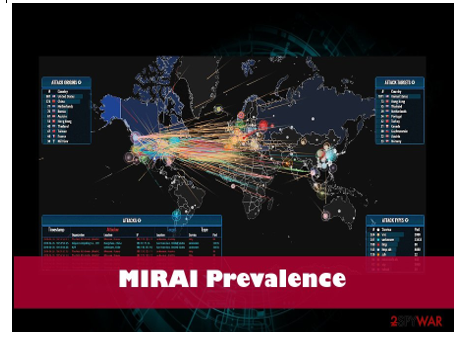
\includegraphics[height=1.2in,width=\columnwidth,trim={0 0 0 0},clip]{images/mirai}
			};              
		}
		\end{tikzpicture}
		\onslide<3->
	\end{figure}
\end{column}

	\begin{column}{0.3\textwidth}
		\begin{figure}
			\begin{tikzpicture}
			\only<4->
			{
				\node [inner sep=-10pt]
				{
					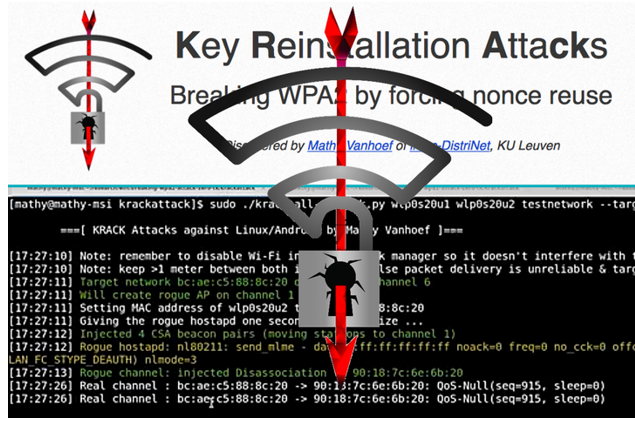
\includegraphics[height=1.2in,width=\columnwidth,trim={0 0 0 0},clip]{images/wifis}
				};
			}
			\end{tikzpicture} 
			\onslide<4->
			
		\end{figure}
	\end{column}            
\end{columns}
\textbf{}\\

\textbf{}\\

\uncover<5->{
\begin{alertblock}{Une Priorité}
%par consequent,
Diminuer les risques de sécurité notamment ceux dû aux attaques \textbf{DDoS} révèle d'une priorité primordiale aussi bien pour les entreprises que pour les opérateurs.
\end{alertblock}}
\end{frame}

\subsection{Objectif}
\begin{frame}
    \frametitle{Objectif}
    \begin{block}{L'objectif principal}
    %Dans ce contexte notre objectif se focalise
     Réaliser une approche résiliente pour l’identification et la détection des attaques DDoS dans les réseaux IoT en vue d'empêcher les intrusions.\\
L'idée Consiste à intégrer l'IA plus precisement le DL afin d'avoir une precision de détection efficace. \\
Par ailleurs cette approche inclue l’utilisation séquentielle de l’auto-encodeur(AE) et des réseaux de neurones profonds(DNN).
\end{block}     
   
\end{frame}

\section{APERÇU SUR L'\'ETAT DE L'ART}
\subsection{IoT}
\begin{frame}{\textbf{IoT}}
\framesubtitle{Définitions}
\begin{minipage}{0.6\textwidth}
	\begin{block}{Définitions}
	\begin{itemize}
	\item<1-> L’Internet des Objets est défini comme un ensemble d'objets inter connectés, disponibles et offrant des services en permanence à travers l’internet.
	\item<2-> Un Objet connecté est un appareil possédant la capacité d’échanger des données via internet avec d’autres entités physiques ou numériques.
	%\item<3-> Exemples d'Objets Connectés : les montres, les réfrigerateurs, les voitures etc.
	\end{itemize}
	\end{block}
\end{minipage}
\begin{minipage}{2cm}

\end{minipage}
\begin{minipage}{0.3\textwidth}
	 	\only<2->{
	    \begin{figure}[t]
 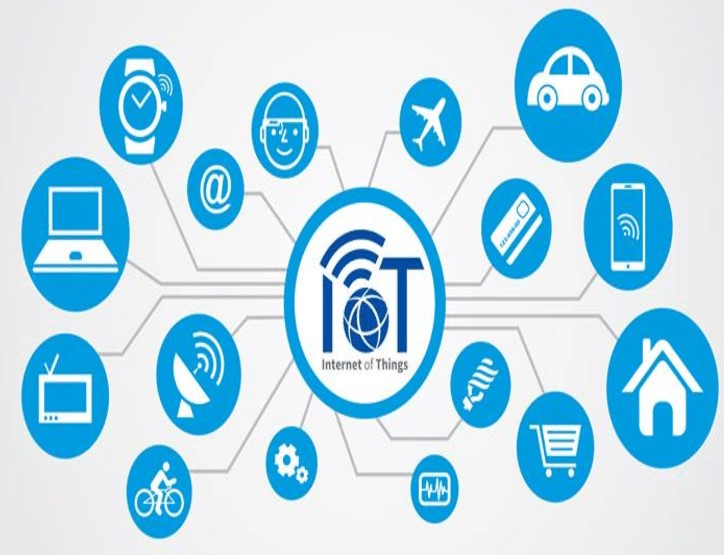
\includegraphics[height=0.6\textheight]{images/IoTI}
	    \end{figure}   
      	} 
\end{minipage}	
\end{frame}
\begin{frame}{\textbf{IoT}}
 %\frametitle{Frametitle}
  %\framesubtitle{Framesubtitle}
\framesubtitle{\textbf{Domaines d'applications}}
\begin{columns}
     \begin{column}{0.4\textwidth}
	    \begin{figure}[t]
	      \centering
	      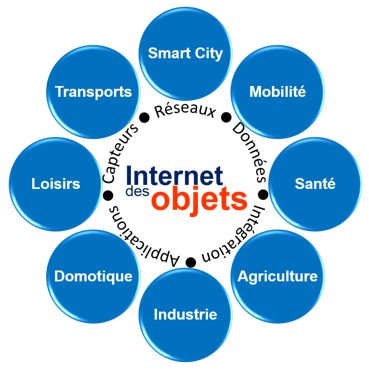
\includegraphics[height=0.7\textheight]{images/Application_IoT}
	    \end{figure}    			
      \end{column}
	  \begin{column}{0.6\textwidth}
      	\only<2->
	      		{
	      \begin{block}{\textbf{Exemples}}
	      	\begin{itemize}
	   	\item<3-> Villes intelligentes : Singapour, Oslo%, Barcelone
  			  			
	    \item<4-> Mobilité : voiture connectée
	      			 				
	    \item<5-> Santé : Tensiomètre connecté, %Oxymètre connecté 
	      			
	      \item<6-> Agriculture : Drones agricoles,%automatisation des serres
	
	      	\item<7-> Industrie : Robot connecté
	      	
	      	\item<8-> Domotique :  Réfrigérateur connecté %Ampoule connecté,
	      		\item<9-> Loisirs : Télévision connectée 
	      		\item<10-> Transports : Gestion de la circulation
	      			\end{itemize}
	      		\end{block}
      		  }
	      	\end{column}
      	\end{columns}	
		 
\end{frame}

\begin{frame}{\textbf{IoT}}
 %\frametitle{Frametitle}
  %\framesubtitle{Framesubtitle}
\framesubtitle{\textbf{Avantages et Inconvénients de l'IoT}}
\framesubtitle{}
	     \begin{columns}
     \begin{column}{0.5\textwidth}
      	\only<1->
	      		{
	      \begin{block}{\textbf{Avantages}}
	      	\begin{itemize}
	   	\item Amélioration de la productivité
  			  			
	    \item Amélioration de nos quotidiens
	      			 				
	    \item Diminution des erreurs humaines 
	      			
	      \item Sécurisation des domiciles 
	
	      	\item Surveillance de sa santé
	      	
	      	\item Aide aux personnes âgées
	      			\end{itemize}
	      		\end{block}
      		  }
	      	\end{column}
	  \begin{column}{0.5\textwidth}
      	\only<2->
	      		{
	      \begin{alertblock}{\textbf{Inconvénients}}
	      	\begin{itemize}
			  	
	    \item Gestion complexe de la \textcolor{red}{sécurité} des objets et des données 
	      			 				
	    \item Interopérabilité et hétérogénéité
	      	\item Génération d'une grande masse de données 		
	      \item  Faible protection de la vie privée
	      			\end{itemize}
	      		\end{alertblock}
      		  }
	      	\end{column}
      	\end{columns}	
\end{frame}

\subsection{DDoS}
\begin{frame}{DDoS}
\begin{columns}
	\begin{column}{0.4\textwidth}
      	\only<1->
	      		{\begin{block}{Définition}
 Le \textbf{DDoS} est l'attaque visant à rendre un service ou une ressource indisponible à ses utilisateurs légitimes. Elle est mise en œuvre à travers un botnet c'est à dire un réseau d'objets infectés
	\end{block}
      		  }
	     \end{column}
     \begin{column}{0.6\textwidth}
      	\only<2->{
	    \begin{figure}[t]
	      \centering
	      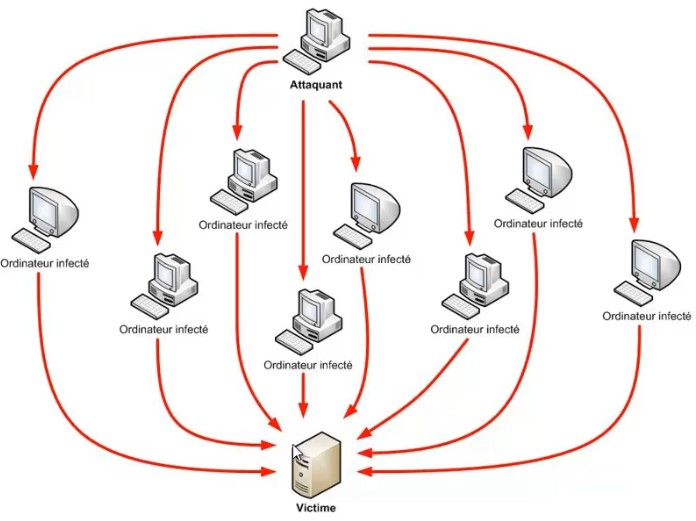
\includegraphics[height=0.8\textheight]{images/Architecture_attaque_DDoS_j}
	    \end{figure}   
      	}   			
      \end{column}
      	\end{columns}	
\end{frame}
\begin{frame}{DDoS}
	
	\begin{block}{Chronologie des attaques DDoS}
	\begin{figure}[t]
	      \centering
	      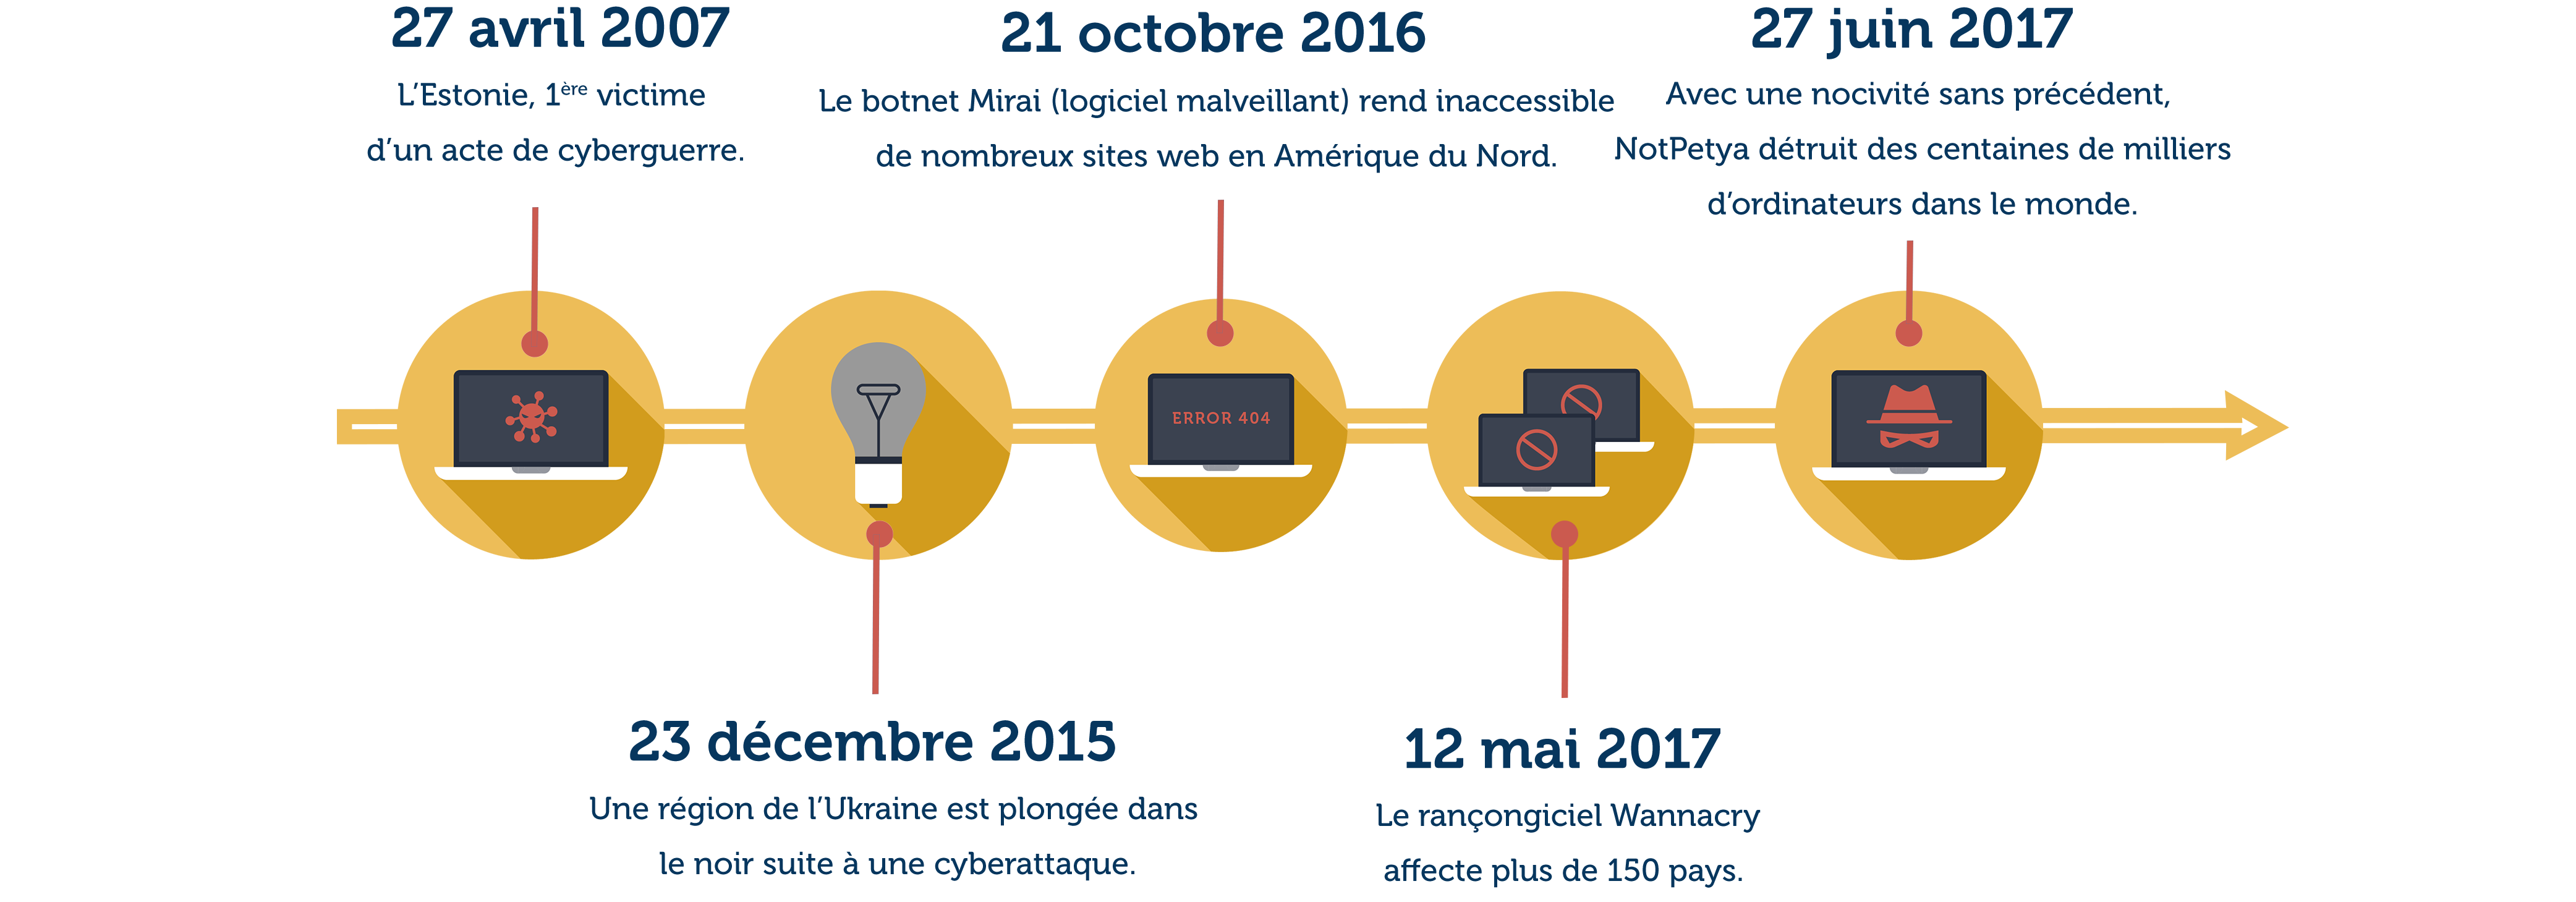
\includegraphics[height=0.6\textheight, width=\textwidth]{images/cybermenace-avis-de-tempete-attaquants-chronologie_1}
	    \end{figure} 
	\end{block}
			
		\end{frame}
%\begin{frame}{DDoS}
	%begin{alertblock}{impact financier}
			%	Selon une étude du FMI en 2018, %les pertes annuelles moyennes dûes aux cyberattaques dépasseraient les 100 milliards de dollars \cite{fmi}.
		%	\end{alertblock}
%\end{frame}

\subsection{IDS}
\begin{frame}
  \frametitle{IDS}
  \begin{block}{Solution pour se protéger contre les attaques DDoS}
  \justifying
  Une méthode efficace pour protéger les réseaux IoT contre les attaques DDoS est de détecter les attaques et de se défendre avant même qu’elles ne se produisent : \pause \textcolor{red}{utilisation des Systèmes de Détection d'Intrusion(IDS)}
  \end{block}
\end{frame}

\begin{frame}
  \frametitle{IDS}
  \framesubtitle{Définition et les différents types d'IDS}
\begin{columns}
	\begin{column}{0.5\textwidth}
			\begin{block}{Définition}
\justifying  
Un IDS est un composant logiciel ou matériel spécialisé,dont le rôle est de surveiller l’activité d’un réseau ou d’un hôte en vue de détecter toute effraction
dans l’utilisation des ressources.
 	 		\end{block}
	 \end{column}
    \begin{column}{0.5\textwidth}
      	\only<2->{
      \begin{block}{Les Différents types d'IDS}
      	\begin{figure}[t]
	       \centering
	     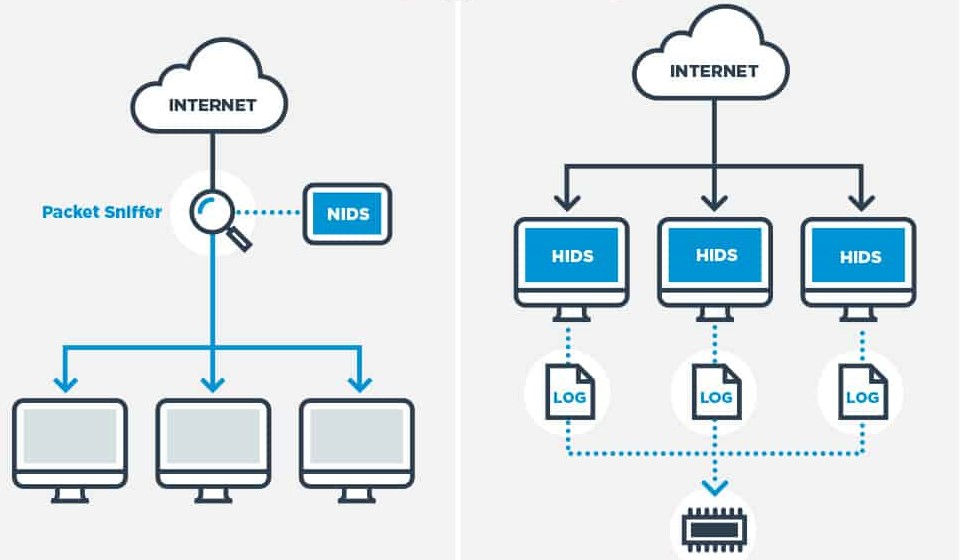
\includegraphics[height=0.6\textheight, width=\textwidth]{images/NIDS-vs-HIDS}
	    \end{figure}
     \end{block}
	     }   			
   \end{column}
\end{columns}  
\end{frame}
\section{CONTRIBUTIONS}
\subsection{Deep Learning}
\begin{frame}
\frametitle{Deep Learning}
\justifying
\begin{block}{Deep Learning}
%les IDS ont été construits sur la base de techniques classiques de machine-learning et data-mining, de modèles basés sur des règles, d'approches d'intelligence artificielle et de modèles statistiques.
%Cependant, ces méthodes produisent souvent des taux de faux positifs (FPR) élevés en raison du chevauchement entre les observations légitimes et anormales. 
L'application des techniques d'apprentissage profond pour la détection d'intrusion donne des Résultats très efficaces par rapport aux IDS classiques.
\begin{itemize}
	\item Taux de détection élevés,
	\item Moins de faux positifs 
\end{itemize}
%de  très efficace %, car elle peut traiter une dimensionnalité élevée et déterminer la structure sous-jacente à partir de données non étiquetées. 
%Plus important encore, lors de la phase d'apprentissage, il effectue un processus d'apprentissage consécutif à l'aide de l'algorithme DAE (Deep Auto-Encoder) non supervisé pour apprendre les comportements normaux du réseau et produire les paramètres optimaux (c-à-d les poids et les biais). 
%Ensuite, un modèle de réseau neuronal profond (DNN) supervisé standard utilise les paramètres estimés des modèles DAE pour régler efficacement ses paramètres et classer les observations de réseau.
%Pour la mise en oeuvre de notre approche nous combinons les deux 
\end{block}
%Une technique d'apprentissage en profondeur est très efficace, car elle peut traiter une dimensionnalité élevée et déterminer la structure sous-jacente à partir de données non étiquetées. 
%Plus important encore, lors de la phase d'apprentissage, il effectue un processus d'apprentissage consécutif à l'aide de l'algorithme DAE (Deep Auto-Encoder) non supervisé pour apprendre les comportements normaux du réseau et produire les paramètres optimaux (c-à-d les poids et les biais). 
%Ensuite, un modèle de réseau neuronal profond (DNN) supervisé standard utilise les paramètres estimés des modèles DAE pour régler efficacement ses paramètres et classer les observations de réseau.
\end{frame}

\subsection{Approche proposée}
\begin{frame}
   \frametitle{Approche proposée}
  \framesubtitle{Architecture du modèle}
  	\begin{figure}[t]
	       \centering
	       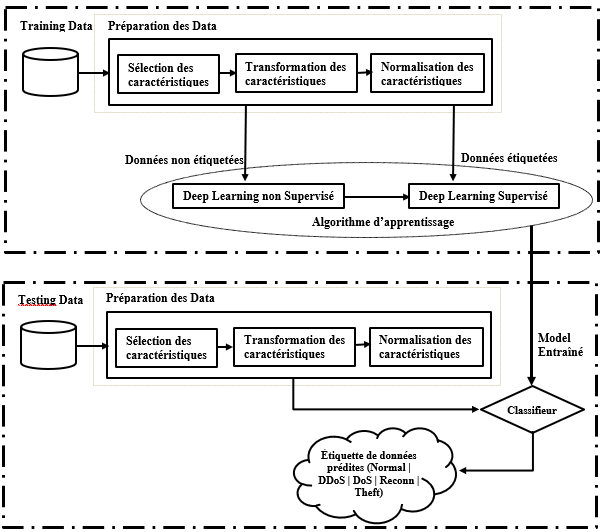
\includegraphics[height=0.8\textheight]{images/architecture}
	    \end{figure}
  
\end{frame}
\begin{frame}
\frametitle{Approche proposée}
\framesubtitle{Choix du Dataset}
\setbeamercovered{transparent}
\begin{minipage}{0.3\textwidth}
	\begin{block}{Datasets}
		\begin{enumerate}
			 \item<1> Bot IoT
			 \item<2> NSL-KDD  
		\end{enumerate}
	\end{block}
\end{minipage}
\textbf{}
\begin{minipage}{0.6\textwidth}
\only<1>{
  	\begin{figure}[t]
	       \centering
 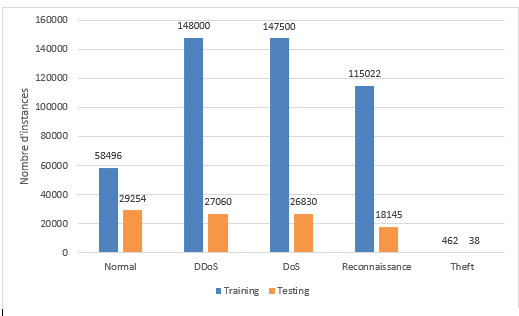
\includegraphics[height=0.8\textheight]{images/graphe}
	    \end{figure}
	    }
	  \only<2>{ 
	    \begin{figure}[t]
	       \centering
 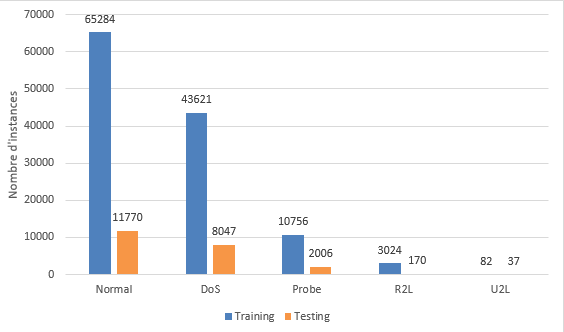
\includegraphics[height=0.8\textheight]{images/grapheNSLKDD}
	    \end{figure}
	    }
\end{minipage}
\setbeamercovered{invisible}
\end{frame} 

\begin{frame}{Approche proposée}
	\framesubtitle{Définition du modèle Auto Encodeur(AE) }
\begin{minipage}{0.4\textwidth}
	\begin{figure}[t]
	       \centering
 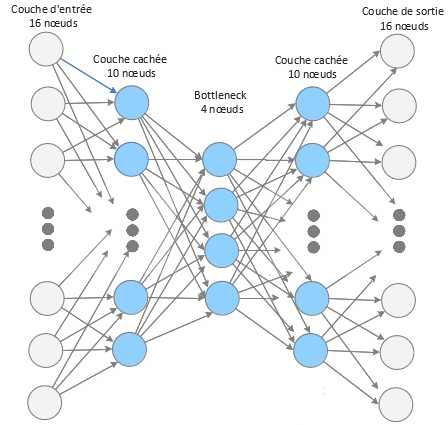
\includegraphics[height=0.7\textheight]{images/ModelAE}
	    \end{figure}
\end{minipage}
\pause{
	\begin{minipage}{0.5\textwidth}
  	\begin{figure}[t]
	     \centering
 	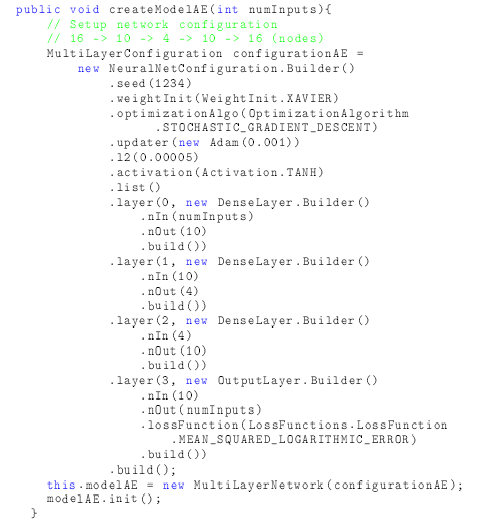
\includegraphics[height=0.8\textheight]{images/codeAE}
 \end{figure}
\end{minipage}
}
\end{frame}

\begin{frame}[fragile]
	\frametitle{Approche proposée}
	\framesubtitle{Définition du modèle du réseau de neurone profond(DNN)}
\begin{minipage}{0.4\textwidth}
\begin{figure}[t]
	       \centering
 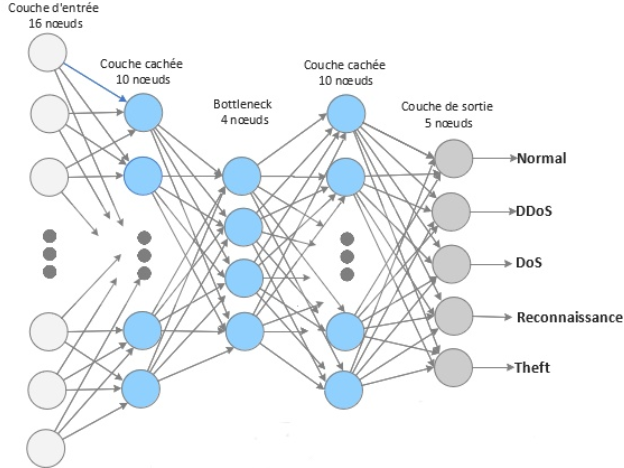
\includegraphics[height=0.7\textheight]{images/ModelDNN}
	    \end{figure}
\end{minipage}
\hspace{0.5cm}
 \pause{
\begin{minipage}{0.5\textwidth}
\lstset{
		tabsize=1,
		%numbers=left,
		commentstyle=\color{green},
		keywordstyle=\color{blue},
		stringstyle=\color{red}	
	}
  	\begin{lstlisting}[language=Java,  basicstyle=\tiny]
		public void createModelFFNN(MultiLayerNetwork modelAE){
        FineTuneConfiguration fineTuneConf = 
        		new FineTuneConfiguration.Builder()
                .updater(new Adam(0.01))
                .build();

        this.modelFFNN = new TransferLearning.Builder(modelAE)
                .fineTuneConfiguration(fineTuneConf)
                .removeOutputLayer()
                .addLayer(new OutputLayer.Builder()
                		.nIn(10)
                		.nOut(this.numClasses)
                		.activation(Activation.SOFTMAX)
                		.lossFunction(new LossMCXENT())
                		.build())
                .build();
        		modelFFNN.init();
    	}
    }
	\end{lstlisting}	
\end{minipage}
   }
\end{frame}

\begin{frame}{Approche proposée}
	\framesubtitle{Fonction d'activation du modèle Auto Encodeur(AE)}
\setbeamercovered{transparent}
\begin{minipage}{0.5\textwidth}
\only<1-2>{
  	\begin{figure}[t]
	       \centering
 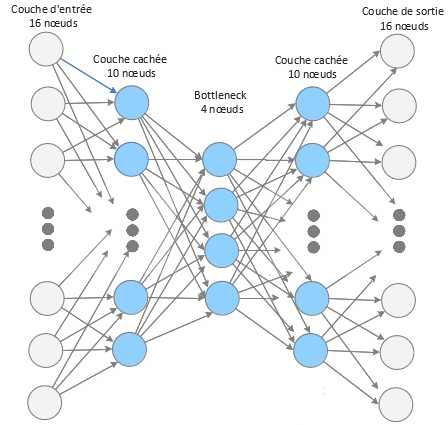
\includegraphics[height=0.8\textheight]{images/ModelAE}
	    \end{figure}
	    }
\end{minipage}
\textbf{}
\begin{minipage}{0.4\textwidth}
	\begin{block}{Fonctions d'activation}
		\begin{enumerate}
			 \item<1> {	
	$$\text{tanh}(x)= \frac{e^{x}-e^{-x}}{e^{x}+e^{-x}}$$
					 }
			 \item<2> {
	$$\text{Softmax}(x_i) = \frac{e^{x_i}}{\sum_{j=1}^k e^{x_j}}$$
 			}
		\end{enumerate} 
	\end{block}
\end{minipage}
\setbeamercovered{invisible}
\end{frame}
  
\begin{frame}{Approche proposée}
	\framesubtitle{Fonction d'activation du modèle du réseau de neurone profond (DNN)}
\setbeamercovered{transparent}
\begin{minipage}{0.5\textwidth}
\only<1-2>{
  	\begin{figure}[t]
	       \centering
 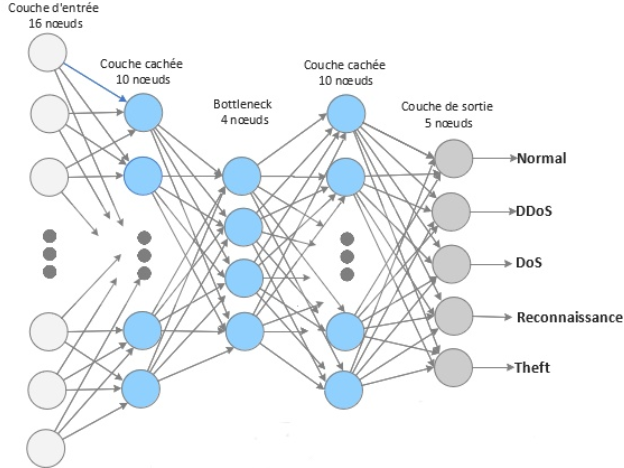
\includegraphics[height=0.7\textheight]{images/ModelDNN}
	    \end{figure}
	    }
\end{minipage}
\vspace{0.1cm}
\begin{minipage}{0.4\textwidth}
	\begin{block}{Fonctions d'activations}
	\begin{enumerate}
			 \item<1> {	
	$$\text{tanh}(x)= \frac{e^{x}-e^{-x}}{e^{x}+e^{-x}}$$
					 }
			 \item<2> {
	$$\text{Softmax}(x_i) = \frac{e^{x_i}}{\sum_{j=1}^k e^{x_j}}$$
 			}
		\end{enumerate}
	\end{block}
\end{minipage}
\setbeamercovered{invisible}
\end{frame} 

\begin{frame}{Approche proposée}
	\framesubtitle{Entrainement du modèle}
\begin{minipage}{0.5\textwidth}
	\begin{figure}[t]
	       \centering
 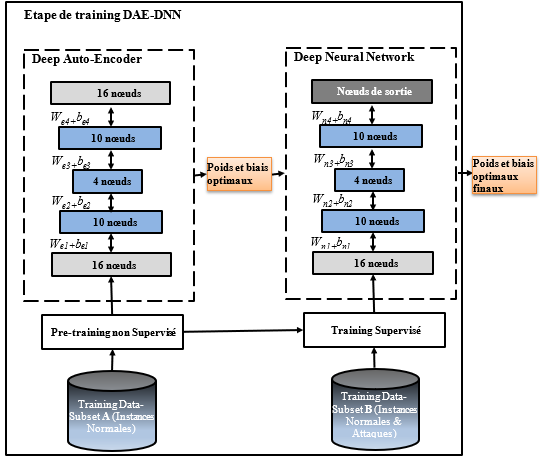
\includegraphics[height=0.7\textheight]{images/Training}
 			\caption{Entraînement du modèle}
	    \end{figure}
\end{minipage}
	\begin{minipage}{0.3\textwidth}
  	\begin{block}{\text{Somme pondérée}}
	 $$z = \sum_{i=1}^n (X_i \times W_i) + bias$$
	$$y = \varphi (z)$$
	\end{block}
\end{minipage}
\end{frame} 

\begin{frame}{Approche proposée}
	\framesubtitle{Phase de test du modèle}
	\begin{minipage}{0.5\textwidth}
  	\begin{figure}[t]
	       \centering
 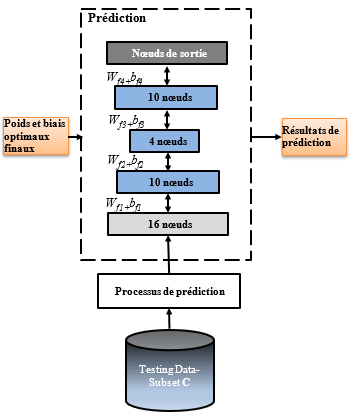
\includegraphics[height=0.7\textheight]{images/testing}
	    \end{figure}
\end{minipage}
	\begin{minipage}{0.3\textwidth}
  	\begin{block}{\text{Somme pondérée}}
	 $$z = \sum_{i=1}^n (X_i \times W_i) + bias$$
	$$y = \varphi (z)$$
	\end{block}
\end{minipage}
\end{frame} 

\begin{frame}{Approche proposée}
	\framesubtitle{Entrainement et test du modèle }
\begin{minipage}{0.4\textwidth}
	\begin{figure}[t]
	       \centering
 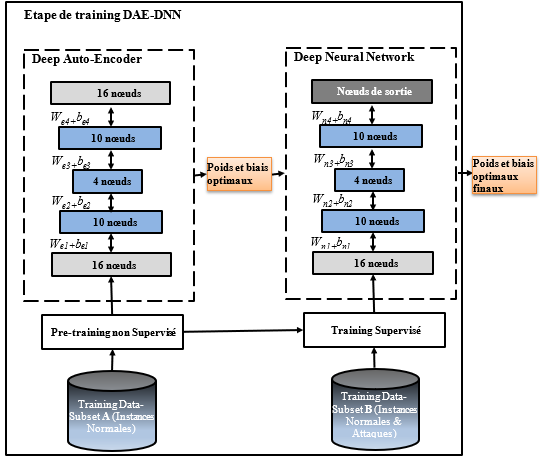
\includegraphics[height=0.7\textheight]{images/Training}
 			\caption{Entraînement du modèle}
	    \end{figure}
\end{minipage}
	\begin{minipage}{0.5\textwidth}
  	\begin{figure}[t]
	       \centering
 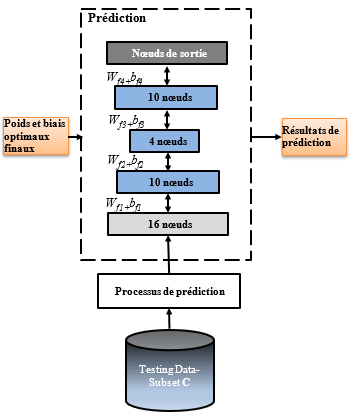
\includegraphics[height=0.7\textheight]{images/testing}
 			\caption{Phase de test du modèle} 
	    \end{figure}
\end{minipage}
\end{frame}

\subsection{Résultats}
\begin{frame}
  \frametitle{Résultats}
	\begin{block}{Matrice de confusion}
		\begin{table}[H]
\begin{tabular}{ccccccc}
  \toprule
    \multirow{2}{*}{} & \multicolumn{6}{c}{\textbf{Classe prédite}} \\
    \cmidrule{2-7} & \textbf{Classifié}	$\longrightarrow$ & \textbf{Normal} & \textbf{DDoS} & \textbf{DoS} & \textbf{Reconn}& \textbf{Theft} \\
  \midrule
    \multirow{5}{*}{\textbf{Classe réelle}} & \textbf{Normal} & 29238 & 1 & 4 & 11 & 0\\
    \cmidrule{2-7}            & \textbf{DDOS} & 0 & 26684  & 357 & 19 & 0 \\
    \cmidrule{2-7}            & \textbf{DOS} & 0 & 718 & 26033 & 79 & 0  \\
    \cmidrule{2-7}            & \textbf{Reconn} & 2 & 59 & 175 & 17909 & 0 \\
    \cmidrule{2-7}            & \textbf{Theft} & 0 & 0 & 0 & 13 & 25\\
  \bottomrule
\end{tabular}
\end{table}
	\end{block}
\end{frame}
\begin{frame}{Résultats}
	\framesubtitle{Métriques d'évaluation}
	\begin{minipage}{0.6\textwidth}
		\begin{figure}[t]
	       \centering
 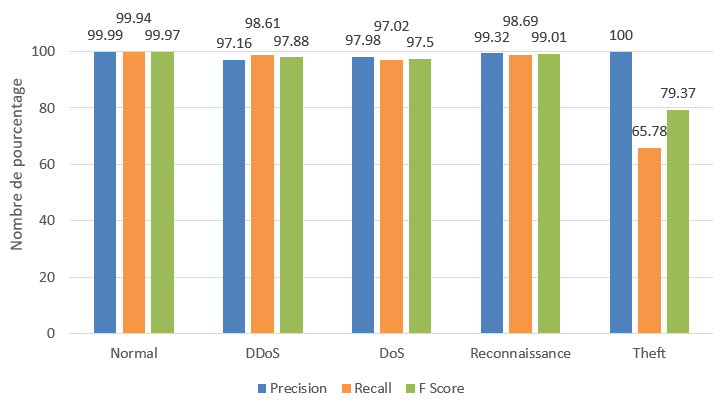
\includegraphics[height=0.7\textheight]{images/resultat} 
	    \end{figure}
	\end{minipage}
	\hspace{1cm}
	\begin{minipage}{0.3\textwidth}
	\pause{
\begin{block}{moyennes des résultats obtenues}
	Accuracy  =  98.58\% \\

	Precision =  98.89\% \\	

	Recall     =  92.01\% \\

	F Score   =  94.74\% \\
	FPR      =  0.38\%\\
\end{block}
	}
	\end{minipage}
\end{frame}
\subsection{Comparaison}
\begin{frame}{Comparaison}
	\begin{block}{Comparaison avec d'autres Travaux}
%\begin{table}[H]
\resizebox{\columnwidth}{!}{%
\begin{tabular}{l c c c}
  \toprule
   \textbf{Méthodes} \& Auteurs & \textbf{L'année} & \textbf{Dataset} & \textbf{Accuracy(taux de reussite)}\\
   \midrule
   \textbf{CNN} \small par B.Susilo et R.Sari & 2020 & Bot IoT & 91.27\% \\
     \textbf{FNN} \small par O.Ibitoye et O.Safig & 2019 & Bot IoT & 95.1\%  \\
    \textbf{CNN} \small par Y.Zheng, Y.Xin et Y.Zhao & 2020 & NSLKDD & 86.95\%  \\
     \textbf{MLP} \small par MOKHTARI Sidi  & 2018 & NSL-KDD  & 93.57\%  \\
\midrule  
\multirow{2}{*}{\textbf{Notre Approche}}&\multirow{2}{*}{2020}&Bot IoT & 98.58\% \\
 \cmidrule{3-4} 											&{}& NSL-KDD & 99.12\% \\
  \bottomrule
\end{tabular}
}
%\caption{comparaison de notre approche avec d'autres approches dans la littérature}
%\label{tab3}
%\end{table} 
	\end{block}
\end{frame}
\section{CONCLUSION G\'EN\'ERALE}
\subsection{Conclusion}
\begin{frame}{Conclusion}
\begin{block}{conclusion}
Notre approche a été testé et validé sur les datasets IoT Botnet
et NSL-KDD pour l’apprentissage et le test. Les résultats obtenus sont très satisfaisants et prouvent l’efficacité de notre approche avec un taux de réussite(Accuracy) de \textbf{98.58\% } et un taux de faux positifs de \textbf{0.38\%}
\end{block}
\end{frame}
\subsection{Perspectives}
\begin{frame}{Perspectives}
\begin{itemize}
\item IDS mode online 
\item Gestion multi tâches des alertes dans l’IDS 
\item Générer et Tester avec son propre dataset 
\end{itemize}
\end{frame}
\begin{frame}[plain,c]
    \begin{center}
    \Huge Merci pour votre attention!
    \end{center}
\end{frame}

\end{document}
